% ============================================================
% LLM Building Blocks: 5 Topics, 1 Anchor
% "The cat sat on the ___" -- 30 Slides
% Standalone Beamer file
% ============================================================
\documentclass[aspectratio=169,12pt]{beamer}

% ---- Theme & Colors ----
\usetheme{Madrid}
\usecolortheme{whale}

% Custom color palette
\definecolor{babylonBrown}{RGB}{139,90,43}
\definecolor{greekBlue}{RGB}{0,71,171}
\definecolor{indianSaffron}{RGB}{204,119,34}
\definecolor{chineseRed}{RGB}{170,56,30}
\definecolor{islamicGreen}{RGB}{0,128,55}
\definecolor{medievalPurple}{RGB}{102,51,153}
\definecolor{renaissanceGold}{RGB}{184,134,11}
\definecolor{enlightenmentTeal}{RGB}{0,128,128}
\definecolor{modernSteel}{RGB}{70,130,180}
\definecolor{digitalBlue}{RGB}{30,80,162}
\definecolor{aiViolet}{RGB}{106,13,173}
\definecolor{accentOrange}{RGB}{230,126,34}
\definecolor{darkBg}{RGB}{30,30,30}

% LLM-specific section colors
\definecolor{linalgTeal}{RGB}{0,150,136}
\definecolor{calculusRed}{RGB}{211,47,47}
\definecolor{probBlue}{RGB}{25,118,210}
\definecolor{infoAmber}{RGB}{255,160,0}
\definecolor{logicGray}{RGB}{97,97,97}
\definecolor{approxGreen}{RGB}{56,142,60}
\definecolor{neuronPink}{RGB}{194,24,91}
\definecolor{seqIndigo}{RGB}{63,81,181}

% Set main beamer colors
\setbeamercolor{palette primary}{bg=aiViolet,fg=white}
\setbeamercolor{palette secondary}{bg=aiViolet!80,fg=white}
\setbeamercolor{palette tertiary}{bg=aiViolet!60,fg=white}
\setbeamercolor{frametitle}{bg=aiViolet,fg=white}
\setbeamercolor{title}{bg=aiViolet,fg=white}
\setbeamercolor{section in toc}{fg=aiViolet}
\setbeamercolor{block title}{bg=aiViolet,fg=white}
\setbeamercolor{block body}{bg=aiViolet!5}
\setbeamercolor{item}{fg=aiViolet}

% ---- Fonts ----
\usefonttheme{professionalfonts}
\setbeamerfont{title}{size=\Large,series=\bfseries}
\setbeamerfont{frametitle}{size=\large,series=\bfseries}
\setbeamerfont{framesubtitle}{size=\normalsize,series=\mdseries}

% ---- Packages ----
\usepackage[utf8]{inputenc}
\usepackage[T1]{fontenc}
\usepackage{amsmath,amssymb,amsfonts}
\usepackage{graphicx}
\usepackage{tikz}
\usetikzlibrary{shapes,arrows.meta,positioning,calc,decorations.pathmorphing,backgrounds,fit}
\usepackage{booktabs}
\usepackage{multicol}
\usepackage{hyperref}
\usepackage{fontawesome5}
\usepackage{xcolor}
\usepackage{pgfplots}
\pgfplotsset{compat=1.18}
\usepackage{tcolorbox}
\tcbuselibrary{skins,breakable}

% ---- Custom Commands ----

% Person info box
\newtcolorbox{personbox}[2][]{%
  colback=#2!5,
  colframe=#2,
  fonttitle=\bfseries,
  title=#1,
  rounded corners,
  boxrule=1pt,
  left=4pt,right=4pt,top=4pt,bottom=4pt
}

% Key insight callout
\newtcolorbox{insightbox}{%
  colback=accentOrange!10,
  colframe=accentOrange,
  fonttitle=\bfseries,
  title={\faLightbulb\ Key Insight},
  rounded corners,
  boxrule=1pt,
  left=4pt,right=4pt,top=4pt,bottom=4pt
}

% Connection to LLM callout
\newtcolorbox{llmconnection}{%
  colback=aiViolet!8,
  colframe=aiViolet,
  fonttitle=\bfseries,
  title={\faRobot\ Inside the LLM},
  rounded corners,
  boxrule=1pt,
  left=4pt,right=4pt,top=4pt,bottom=4pt
}

% Progress bar (5 topics)
\newcommand{\progressbar}[1]{%
  \begin{center}\small\textbf{Topics explored: #1 / 5}\hspace{6pt}%
  \ifnum#1>0\textcolor{linalgTeal}{\rule{10pt}{10pt}}\else\textcolor{gray!30}{\rule{10pt}{10pt}}\fi\hspace{2pt}%
  \ifnum#1>1\textcolor{probBlue}{\rule{10pt}{10pt}}\else\textcolor{gray!30}{\rule{10pt}{10pt}}\fi\hspace{2pt}%
  \ifnum#1>2\textcolor{calculusRed}{\rule{10pt}{10pt}}\else\textcolor{gray!30}{\rule{10pt}{10pt}}\fi\hspace{2pt}%
  \ifnum#1>3\textcolor{seqIndigo}{\rule{10pt}{10pt}}\else\textcolor{gray!30}{\rule{10pt}{10pt}}\fi\hspace{2pt}%
  \ifnum#1>4\textcolor{neuronPink}{\rule{10pt}{10pt}}\else\textcolor{gray!30}{\rule{10pt}{10pt}}\fi%
  \end{center}%
}

% Topic question box
\newcommand{\topicquestion}[2]{%
  \begin{tcolorbox}[colframe=#1, colback=#1!5, boxrule=1.5pt, arc=4pt]
    \centering
    {\large\textbf{``The cat sat on the \rule{1.5cm}{0.4pt}''}}\\[8pt]
    {\normalsize\textit{#2}}
  \end{tcolorbox}%
}

% Verify tag (for speaker notes)
\newcommand{\verifytag}[1]{\textcolor{red!70}{\textbf{[VERIFY:} \textit{#1}\textbf{]}}}

% Slide counter in footline
\setbeamertemplate{footline}{%
  \leavevmode%
  \hbox{%
    \begin{beamercolorbox}[wd=.333333\paperwidth,ht=2.25ex,dp=1ex,center]{author in head/foot}%
      \usebeamerfont{author in head/foot}\insertshortauthor
    \end{beamercolorbox}%
    \begin{beamercolorbox}[wd=.333333\paperwidth,ht=2.25ex,dp=1ex,center]{title in head/foot}%
      \usebeamerfont{title in head/foot}\insertshorttitle
    \end{beamercolorbox}%
    \begin{beamercolorbox}[wd=.333333\paperwidth,ht=2.25ex,dp=1ex,right]{date in head/foot}%
      \usebeamerfont{date in head/foot}\insertframenumber{} / \inserttotalframenumber\hspace*{2ex}
    \end{beamercolorbox}}%
  \vskip0pt%
}

% Remove navigation symbols
\setbeamertemplate{navigation symbols}{}

% Tighten vertical spacing below frame titles
\addtobeamertemplate{frametitle}{}{\vspace{-0.3em}}

% ---- Document Info ----
\title[5 Topics -- LLM Building Blocks]{The Building Blocks of LLMs\\[0.3em]{\large Five Questions, One Sentence, 2,000 Years of Mathematics}}
\subtitle{From ``The cat sat on the \rule{1cm}{0.4pt}'' to the Transformer}
\author{Prof.\ J.\ Osterrieder}
\date{2026}
\institute{}

% ============================================================
\begin{document}

% ============================================================
% SLIDE 1: Title
% ============================================================
\begin{frame}[plain]
\maketitle
\note{
OPENING: ``This lecture is about one sentence, one question, and the 2,000 years of mathematics that make the answer possible.''

Set scope: we will not cover everything about LLMs. We will take ONE sentence and ask FIVE questions about how the AI handles it.

Each question leads us to specific mathematical inventions, specific people, specific dates. By the end, every piece of the machine will have a name and a story.
}
\end{frame}

% ============================================================
% SLIDE 2: The Anchor
% ============================================================
\begin{frame}{One Sentence. Five Questions.}

\begin{center}
{\LARGE\textbf{``The cat sat on the \rule{2cm}{0.5pt}''}}
\end{center}

\vspace{0.5em}

Every time you use ChatGPT or Claude, the AI is doing \textbf{one thing}: predicting the next word.

\vspace{0.5em}
To play this game, it needs five abilities:

\begin{enumerate}
  \item \textcolor{linalgTeal}{\textbf{How does it know which words are similar?}}
  \item \textcolor{probBlue}{\textbf{How does it choose the next word?}}
  \item \textcolor{calculusRed}{\textbf{How does it learn from mistakes?}}
  \item \textcolor{seqIndigo}{\textbf{How does it understand context?}}
  \item \textcolor{neuronPink}{\textbf{How does it get so good?}}
\end{enumerate}

\vspace{0.3em}
\begin{center}
\small Each was invented by specific people, at specific times, for reasons that had \textbf{nothing to do with AI}.
\end{center}

\note{
``Every time you type something into ChatGPT or Claude, the AI is doing one thing: predicting the next word. `The cat sat on the blank.' That is the entire game. But to play this game, the AI needs five abilities. We will discover them one by one.''

Point to the list. Each lights up in its color as we reach it. By slide 28, all five are lit.

Connection: this IS the anchor. Every subsequent topic returns here.
}
\end{frame}

% ============================================================
% TOPIC 1: How does it know which words are similar?
% Color: linalgTeal  |  Slides 3--7
% ============================================================

% ============================================================
% SLIDE 3: The Question -- Words as Numbers
% ============================================================
\begin{frame}{``The cat sat on the \rule{1.2cm}{0.4pt}'' -- How Does It Know Which Words Are Similar?}

\topicquestion{linalgTeal}{The AI thinks ``mat'' and ``rug'' are good answers, but not ``quantum.'' How does it know which words are similar?}

\vspace{0.3em}

\begin{columns}[T]
\column{0.48\textwidth}
\textbf{Good candidates:}\\[3pt]
\textcolor{linalgTeal}{\faCheck}~mat \quad
\textcolor{linalgTeal}{\faCheck}~rug \quad
\textcolor{linalgTeal}{\faCheck}~carpet\\[6pt]
\textbf{Bad candidate:}\\[3pt]
\textcolor{calculusRed}{\faTimes}~quantum

\column{0.48\textwidth}
\textbf{The secret:} every word is a list of numbers.\\[6pt]
``mat'' = $[0.2,\; 0.8,\; -0.1,\; \ldots]$\\
\hspace{2.4em}{\small(768 numbers)}\\[6pt]
Similar words $\rightarrow$ similar lists.
\end{columns}

\note{
NOW: The AI turns words into lists of numbers -- vectors. Similar words end up as similar lists.

THEN: Three people from the 1800s invented the math for this.

``Let's start with the most basic question. The AI thinks `mat' is a good answer. It also likes `rug' and `carpet.' But not `quantum.' How does it know? The answer: it turns every word into a list of numbers -- a vector. And similar words end up as similar lists.''
}
\end{frame}

% ============================================================
% SLIDE 4: The History -- Grassmann, Cayley, Gibbs
% ============================================================
\begin{frame}{The Inventors of the Number-World}

\begin{columns}[T]
\column{0.32\textwidth}
\begin{tcolorbox}[colframe=linalgTeal, colback=linalgTeal!5, boxrule=1pt,
  fonttitle=\bfseries\small, title={Grassmann, 1844}, left=2pt, right=2pt, top=2pt, bottom=2pt]
\centering\small
A schoolteacher in Prussia.\\[3pt]
Published a book so abstract that \textbf{nobody read it}.\\[3pt]
Invented \textbf{vector spaces} -- the exact structure AI uses.
\end{tcolorbox}

\column{0.32\textwidth}
\begin{tcolorbox}[colframe=linalgTeal, colback=linalgTeal!5, boxrule=1pt,
  fonttitle=\bfseries\small, title={Cayley, 1858}, left=2pt, right=2pt, top=2pt, bottom=2pt]
\centering\small
Sylvester named it ``matrix'' -- Latin for \textit{womb}.\\[3pt]
Cayley defined \textbf{matrix multiplication}.\\[3pt]
Every neural network layer uses it.
\end{tcolorbox}

\column{0.32\textwidth}
\begin{tcolorbox}[colframe=linalgTeal, colback=linalgTeal!5, boxrule=1pt,
  fonttitle=\bfseries\small, title={Gibbs, 1881}, left=2pt, right=2pt, top=2pt, bottom=2pt]
\centering\small
Yale physicist.\\[3pt]
Formalized the \textbf{dot product}.\\[3pt]
Multiply, add, get similarity.\\[3pt]
$\vec{a}\cdot\vec{b} = \sum a_i b_i$
\end{tcolorbox}
\end{columns}

\vspace{0.4em}
\begin{insightbox}
None of them had any idea their math would end up inside your phone.
\end{insightbox}

\note{
THEN: ``Grassmann was a schoolteacher in Prussia. He published a book so abstract that nobody read it. It defined vector spaces. Sylvester, a failed barrister, named the matrix. Gibbs, a physicist at Yale, formalized the dot product.''

NOW: ``These are the tools that let the AI measure `mat' vs.\ `quantum.'''
}
\end{frame}

% ============================================================
% SLIDE 5: The Mechanism -- Embeddings and the Dot Product
% ============================================================
\begin{frame}{Words Live in a Number-World}

\begin{columns}[T]
\column{0.55\textwidth}
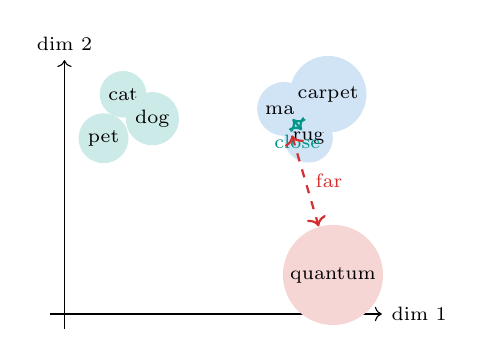
\begin{tikzpicture}[scale=0.62, every node/.style={font=\scriptsize}]
  % Axes
  \draw[->] (-0.3,0) -- (6.5,0) node[right] {dim 1};
  \draw[->] (0,-0.3) -- (0,5.2) node[above] {dim 2};
  % Animal cluster
  \node[fill=linalgTeal!20, circle, inner sep=2pt] (cat) at (1.2,4.5) {cat};
  \node[fill=linalgTeal!20, circle, inner sep=2pt] (dog) at (1.8,4.0) {dog};
  \node[fill=linalgTeal!20, circle, inner sep=2pt] (pet) at (0.8,3.6) {pet};
  % Furniture cluster
  \node[fill=probBlue!20, circle, inner sep=2pt] (mat) at (4.5,4.2) {mat};
  \node[fill=probBlue!20, circle, inner sep=2pt] (rug) at (5.0,3.6) {rug};
  \node[fill=probBlue!20, circle, inner sep=2pt] (carpet) at (5.4,4.5) {carpet};
  % Far away
  \node[fill=calculusRed!20, circle, inner sep=2pt] (quantum) at (5.5,0.8) {quantum};
  % Annotation
  \draw[<->, thick, linalgTeal] (mat) -- (rug) node[midway, below, font=\scriptsize] {close};
  \draw[<->, thick, calculusRed, dashed] (mat) -- (quantum) node[midway, right, font=\scriptsize] {far};
\end{tikzpicture}

\column{0.43\textwidth}
\textbf{Dot product = similarity}\\[3pt]
{\small
\begin{tabular}{ll}
$\vec{\text{mat}}\cdot\vec{\text{rug}}$ & $= 0.92$ (similar)\\
$\vec{\text{mat}}\cdot\vec{\text{quantum}}$ & $= 0.03$ (unrelated)\\
\end{tabular}}

\vspace{0.4em}
\textbf{\faHandPointRight~Interactive Moment:}\\[3pt]
\textcolor{linalgTeal}{\textbf{king $-$ man $+$ woman $=$ ?}}\\[4pt]
{\small Mikolov (Word2Vec, 2013): word vector arithmetic works.}\\[3pt]
{\small\textit{``Not a trick. Geometry in 768 dimensions.''}}
\end{columns}

\note{
INTERACTIVE MOMENT 1: ``What does king minus man plus woman equal?'' Collect guesses. Reveal: queen.

``Mikolov showed in 2013 that if you train a neural network to predict words from context, the vectors it learns have astonishing properties. Similar words cluster together. And relationships are preserved as directions: king is to queen as man is to woman.''

``The dot product -- Gibbs's formula from 1881 -- is the similarity measure.''

Bridge: ``Now the AI knows `mat' and `rug' are similar. But which one should it pick?''
}
\end{frame}

% ============================================================
% SLIDE 6: The Mechanism -- Layers as Matrix Multiplications
% ============================================================
\begin{frame}{Every Layer Is a Matrix Multiplication}

\begin{columns}[T]
\column{0.45\textwidth}
\textbf{One layer:}\\[4pt]
$\vec{y} = W \cdot \vec{x} + \vec{b}$\\[6pt]
{\small Input vector $\vec{x}$, weight matrix $W$, bias $\vec{b}$, output $\vec{y}$.}

\vspace{0.5em}
\textbf{A neural network:}\\[4pt]
Stack 96 of these.

\vspace{0.5em}
\begin{insightbox}
Cayley's math from 1858, repeated 96 times, is the engine of modern AI.
\end{insightbox}

\column{0.50\textwidth}
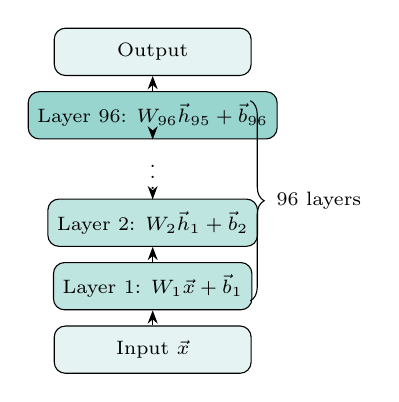
\begin{tikzpicture}[scale=0.62, every node/.style={font=\scriptsize}]
  % Input
  \node[draw, rounded corners, fill=linalgTeal!10, minimum width=2.5cm, minimum height=0.6cm] (in) at (0,0) {Input $\vec{x}$};
  % Layers
  \node[draw, rounded corners, fill=linalgTeal!25, minimum width=2.5cm, minimum height=0.6cm] (l1) at (0,1.3) {Layer 1: $W_1\vec{x}+\vec{b}_1$};
  \node[draw, rounded corners, fill=linalgTeal!25, minimum width=2.5cm, minimum height=0.6cm] (l2) at (0,2.6) {Layer 2: $W_2\vec{h}_1+\vec{b}_2$};
  \node (dots) at (0,3.7) {$\vdots$};
  \node[draw, rounded corners, fill=linalgTeal!40, minimum width=2.5cm, minimum height=0.6cm] (l96) at (0,4.8) {Layer 96: $W_{96}\vec{h}_{95}+\vec{b}_{96}$};
  \node[draw, rounded corners, fill=linalgTeal!10, minimum width=2.5cm, minimum height=0.6cm] (out) at (0,6.1) {Output};
  % Arrows
  \draw[-Stealth] (in) -- (l1);
  \draw[-Stealth] (l1) -- (l2);
  \draw[-Stealth] (l2) -- (dots);
  \draw[-Stealth] (dots) -- (l96);
  \draw[-Stealth] (l96) -- (out);
  % Brace
  \draw[decorate, decoration={brace, amplitude=5pt, mirror}] (2.0,1.0) -- (2.0,5.1) node[midway, right=6pt, font=\scriptsize] {96 layers};
\end{tikzpicture}
\end{columns}

\note{
``Every layer in a neural network does one thing: multiply your data by a matrix and transform it. That is Cayley's matrix multiplication from 1858. Stack 96 of these and you have GPT-4. The math has not changed. The scale has.''

Bridge: ``The AI now has a number-world for words and a way to transform them. But it still needs to pick a word.''
}
\end{frame}

% ============================================================
% SLIDE 7: Inside the LLM -- Where Vectors Live
% ============================================================
\begin{frame}{Building Block Found: Vectors, Matrices, Dot Product}

\begin{columns}[T]
\column{0.55\textwidth}
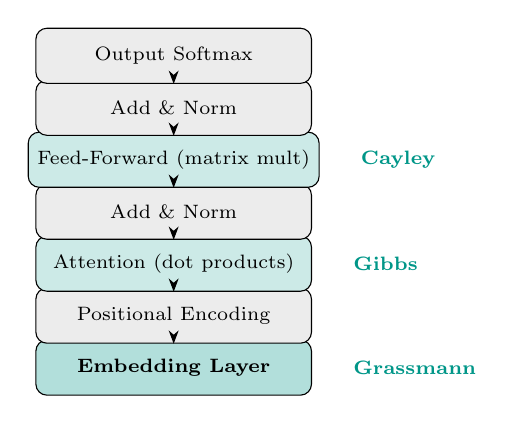
\begin{tikzpicture}[scale=0.55, every node/.style={font=\scriptsize}]
  % Simplified transformer
  \node[draw, fill=linalgTeal!30, rounded corners, minimum width=3.5cm, minimum height=0.7cm]
    (emb) at (0,0) {\textbf{Embedding Layer}};
  \node[draw, fill=gray!15, rounded corners, minimum width=3.5cm, minimum height=0.7cm]
    (pos) at (0,1.2) {Positional Encoding};
  \node[draw, fill=linalgTeal!20, rounded corners, minimum width=3.5cm, minimum height=0.7cm]
    (attn) at (0,2.4) {Attention {\scriptsize(dot products)}};
  \node[draw, fill=gray!15, rounded corners, minimum width=3.5cm, minimum height=0.7cm]
    (an1) at (0,3.6) {Add \& Norm};
  \node[draw, fill=linalgTeal!20, rounded corners, minimum width=3.5cm, minimum height=0.7cm]
    (ff) at (0,4.8) {Feed-Forward {\scriptsize(matrix mult)}};
  \node[draw, fill=gray!15, rounded corners, minimum width=3.5cm, minimum height=0.7cm]
    (an2) at (0,6.0) {Add \& Norm};
  \node[draw, fill=gray!15, rounded corners, minimum width=3.5cm, minimum height=0.7cm]
    (out) at (0,7.2) {Output Softmax};
  % Arrows
  \draw[-Stealth] (emb) -- (pos);
  \draw[-Stealth] (pos) -- (attn);
  \draw[-Stealth] (attn) -- (an1);
  \draw[-Stealth] (an1) -- (ff);
  \draw[-Stealth] (ff) -- (an2);
  \draw[-Stealth] (an2) -- (out);
  % Labels
  \node[right=0.4cm, linalgTeal, font=\scriptsize\bfseries] at (emb.east) {Grassmann};
  \node[right=0.4cm, linalgTeal, font=\scriptsize\bfseries] at (attn.east) {Gibbs};
  \node[right=0.4cm, linalgTeal, font=\scriptsize\bfseries] at (ff.east) {Cayley};
\end{tikzpicture}

\column{0.42\textwidth}
\textbf{Where Topic 1 lives:}
\begin{itemize}
  \item \textcolor{linalgTeal}{\textbf{Embedding layer}} -- words become vectors (Grassmann)
  \item \textcolor{linalgTeal}{\textbf{Attention}} -- dot products measure similarity (Gibbs)
  \item \textcolor{linalgTeal}{\textbf{Every layer}} -- matrix multiplication (Cayley)
\end{itemize}

\vspace{0.5em}
\progressbar{1}

\vspace{0.3em}
\begin{center}
\small\textit{We know which words are similar. Now: how does the AI \textbf{choose}?}
\end{center}
\end{columns}

\note{
``The embedding layer -- that is Grassmann's vector space. Every attention score -- that is Gibbs's dot product. Every layer transformation -- that is Cayley's matrix multiplication.''

``One building block found. Four to go.''

Bridge: ``We know which words are similar. Now: how does the AI CHOOSE?''
}
\end{frame}

% ============================================================
% TOPIC 2: How does it choose the next word?
% Color: probBlue  |  Slides 8--12
% ============================================================

% ============================================================
% SLIDE 8: The Question -- From Scores to Probabilities
% ============================================================
\begin{frame}{``The cat sat on the \rule{1.2cm}{0.4pt}'' -- How Does It Choose the Next Word?}

\topicquestion{probBlue}{The AI has 50,000+ words to choose from. It picks ``mat'' 68\% of the time. How?}

\vspace{0.2em}

\begin{columns}[T]
\column{0.48\textwidth}
\textbf{Raw scores (logits):}\\[3pt]
{\small\begin{tabular}{lr}
mat & $3.2$ \\
floor & $1.8$ \\
table & $1.1$ \\
couch & $0.6$ \\
quantum & $-4.7$ \\
\end{tabular}}

\column{0.48\textwidth}
\textbf{Probabilities (???):}\\[3pt]
{\small\begin{tabular}{lr}
mat & $68\%$ \\
floor & $15\%$ \\
table & $8\%$ \\
couch & $4\%$ \\
quantum & $\approx 0\%$ \\
\end{tabular}}

\vspace{0.3em}
{\small How do raw numbers become a probability distribution?}
\end{columns}

\note{
``Back to our sentence. The AI has processed it through its layers and now has a raw score for every word in its vocabulary -- over 50,000 words. `Mat' scores high. `Quantum' scores low. But these are just numbers, not probabilities. How does it turn scores into a choice?''

This is the second facet of ``predicting the next word.''
}
\end{frame}

% ============================================================
% SLIDE 9: The History -- Pascal, Boltzmann, Shannon
% ============================================================
\begin{frame}{From a Gambling Question to Every Word AI Says}

\begin{columns}[T]
\column{0.32\textwidth}
\begin{tcolorbox}[colframe=probBlue, colback=probBlue!5, boxrule=1pt,
  fonttitle=\bfseries\small, title={Pascal \& Fermat, 1654}, left=2pt, right=2pt, top=2pt, bottom=2pt]
\centering
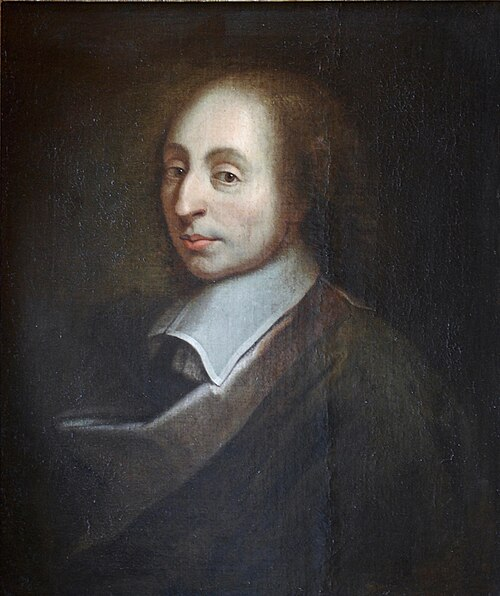
\includegraphics[height=1.2cm]{figures/pascal.jpg}\\[3pt]
{\small A gambler lost at dice and wrote to Pascal.\\[2pt]
Probability was born from a \textbf{letter exchange}.}
\end{tcolorbox}

\column{0.32\textwidth}
\begin{tcolorbox}[colframe=probBlue, colback=probBlue!5, boxrule=1pt,
  fonttitle=\bfseries\small, title={Boltzmann, 1870s}, left=2pt, right=2pt, top=2pt, bottom=2pt]
\centering\small
Studied how gas molecules distribute among energy levels.\\[3pt]
His formula: $\frac{e^{x_i}}{\sum e^{x_j}}$\\[3pt]
\textbf{Now called softmax.}
\end{tcolorbox}

\column{0.32\textwidth}
\begin{tcolorbox}[colframe=probBlue, colback=probBlue!5, boxrule=1pt,
  fonttitle=\bfseries\small, title={Shannon, 1948}, left=2pt, right=2pt, top=2pt, bottom=2pt]
\centering
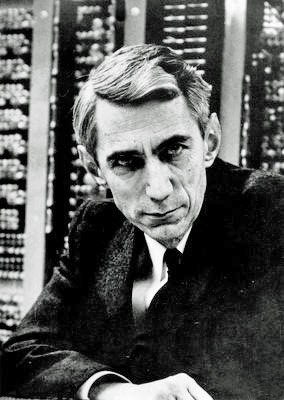
\includegraphics[height=1.2cm]{figures/shannon.jpg}\\[3pt]
{\small Language as statistics.\\[2pt]
\textbf{Cross-entropy}: how to measure prediction quality.}
\end{tcolorbox}
\end{columns}

\vspace{0.3em}
\begin{insightbox}
Pascal's gambling question $\rightarrow$ Boltzmann's gas molecules $\rightarrow$ the AI choosing ``mat.''
\end{insightbox}

\note{
``Probability started because a gambler lost at dice and wrote to Blaise Pascal. Pascal wrote to Fermat. Their letters invented a new branch of mathematics.

Then in the 1870s, Boltzmann studied how gas molecules distribute among energy levels and wrote down a formula: e to the x over the sum of e to the x. That exact formula -- now called softmax -- is how every AI picks every word.

And Shannon, in 1948, showed how to measure whether the predictions are any good.''
}
\end{frame}

% ============================================================
% SLIDE 10: The Mechanism -- Softmax
% ============================================================
\begin{frame}{The Softmax Pipeline}

\begin{center}
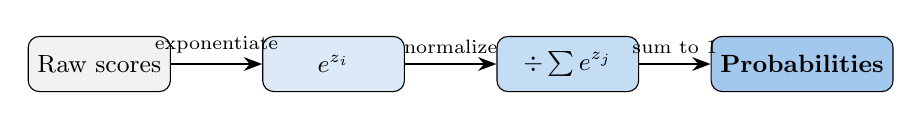
\begin{tikzpicture}[scale=0.85, every node/.style={font=\small}]
  % Pipeline boxes
  \node[draw, fill=gray!10, rounded corners, minimum width=1.8cm, minimum height=0.7cm]
    (raw) at (0,0) {Raw scores};
  \node[draw, fill=probBlue!15, rounded corners, minimum width=1.8cm, minimum height=0.7cm]
    (exp) at (3.5,0) {$e^{z_i}$};
  \node[draw, fill=probBlue!25, rounded corners, minimum width=1.8cm, minimum height=0.7cm]
    (norm) at (7,0) {$\div \sum e^{z_j}$};
  \node[draw, fill=probBlue!40, rounded corners, minimum width=2cm, minimum height=0.7cm]
    (prob) at (10.5,0) {\textbf{Probabilities}};
  \draw[-Stealth, thick] (raw) -- (exp) node[midway, above, font=\scriptsize] {exponentiate};
  \draw[-Stealth, thick] (exp) -- (norm) node[midway, above, font=\scriptsize] {normalize};
  \draw[-Stealth, thick] (norm) -- (prob) node[midway, above, font=\scriptsize] {sum to 1};
\end{tikzpicture}
\end{center}

\vspace{-0.2em}

\begin{columns}[T]
\column{0.50\textwidth}
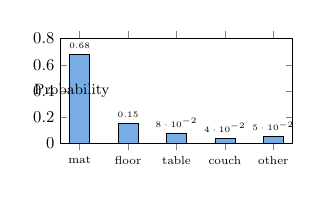
\begin{tikzpicture}[scale=0.60]
\begin{axis}[
    ybar, bar width=12pt,
    ylabel={\small Probability},
    symbolic x coords={mat,floor,table,couch,other},
    xtick=data, xticklabel style={font=\scriptsize},
    ymin=0, ymax=0.8,
    nodes near coords, nodes near coords style={font=\tiny},
    every axis y label/.style={at={(0.05,0.5)}},
    width=6.5cm, height=3.8cm
]
\addplot[fill=probBlue!60] coordinates {(mat,0.68) (floor,0.15) (table,0.08) (couch,0.04) (other,0.05)};
\end{axis}
\end{tikzpicture}

\column{0.46\textwidth}
\vspace{0.3em}
$$\text{softmax}(z_i) = \frac{e^{z_i}}{\displaystyle\sum_{j=1}^{V} e^{z_j}}$$

\vspace{0.3em}
\textbf{\faHandPointRight~Interactive Moment:}\\[2pt]
{\small ``The cat sat on the \rule{1cm}{0.3pt}''\\[2pt]
What word comes next?\\[2pt]
\textit{You and the AI are doing the same thing.}}
\end{columns}

\note{
INTERACTIVE MOMENT 2: ``What word comes next: `The cat sat on the blank'?'' Collect answers from the class. Show the AI's softmax distribution alongside the class's distribution.

``Step 1: exponentiate every score, making them all positive and amplifying differences. Step 2: divide by the total, so they sum to 1. Now they are probabilities. This is Boltzmann's distribution from thermodynamics, applied to words.''

Bridge: ``The AI now picks words. But how does it know if it picked WELL?''
}
\end{frame}

% ============================================================
% SLIDE 11: The Mechanism -- Cross-Entropy
% ============================================================
\begin{frame}{Measuring Mistakes: Cross-Entropy}

\begin{columns}[T]
\column{0.52\textwidth}
\textbf{The correct answer was ``mat.''}

\vspace{0.5em}
\begin{tcolorbox}[colframe=approxGreen, colback=approxGreen!5, boxrule=1pt, left=3pt, right=3pt, top=3pt, bottom=3pt]
\textbf{Scenario A:} AI said ``mat'' with 80\%\\
Loss $= -\log(0.80) = 0.22$ \textcolor{approxGreen}{\faCheck~Good}
\end{tcolorbox}

\vspace{0.3em}
\begin{tcolorbox}[colframe=calculusRed, colback=calculusRed!5, boxrule=1pt, left=3pt, right=3pt, top=3pt, bottom=3pt]
\textbf{Scenario B:} AI said ``mat'' with 5\%\\
Loss $= -\log(0.05) = 3.00$ \textcolor{calculusRed}{\faTimes~Terrible}
\end{tcolorbox}

\column{0.44\textwidth}
\vspace{0.3em}
$$\mathcal{L} = -\log\, p(\text{correct word})$$

\vspace{0.5em}
\textbf{Shannon, 1948:}
\begin{itemize}\small
  \item More surprised by the truth $\rightarrow$ higher loss
  \item Less surprised $\rightarrow$ lower loss
  \item This is the \textbf{only} number the AI tries to minimize
\end{itemize}

\vspace{0.4em}
\begin{insightbox}
Cross-entropy connects \textbf{prediction} (Topic~2) to \textbf{learning} (Topic~3).
\end{insightbox}
\end{columns}

\note{
``Shannon needed a way to measure information. He defined cross-entropy: how surprised you are by the truth, given your predictions. Low surprise = good model. High surprise = bad model.

This number -- cross-entropy loss -- is the ONLY thing the AI tries to minimize during training.

It connects prediction (Topic 2) to learning (Topic 3). Shannon's 1948 formula is the bridge.''

Bridge: ``The AI predicted `mat' but the answer was `rug.' Loss is high. Now it needs to learn from that mistake.''
}
\end{frame}

% ============================================================
% SLIDE 12: Inside the LLM -- Where Probability Lives
% ============================================================
\begin{frame}{Building Block Found: Probability, Softmax, Cross-Entropy}

\begin{columns}[T]
\column{0.55\textwidth}
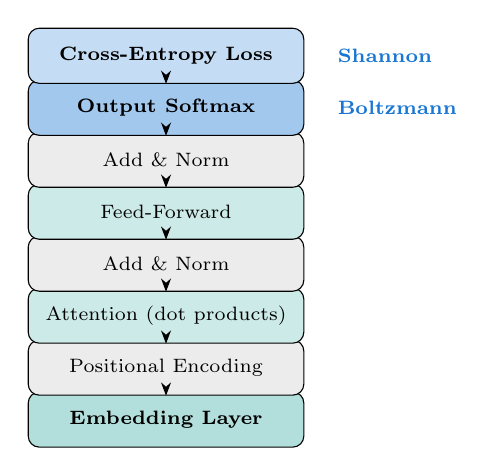
\begin{tikzpicture}[scale=0.55, every node/.style={font=\scriptsize}]
  \node[draw, fill=linalgTeal!30, rounded corners, minimum width=3.5cm, minimum height=0.7cm]
    (emb) at (0,0) {\textbf{Embedding Layer}};
  \node[draw, fill=gray!15, rounded corners, minimum width=3.5cm, minimum height=0.7cm]
    (pos) at (0,1.2) {Positional Encoding};
  \node[draw, fill=linalgTeal!20, rounded corners, minimum width=3.5cm, minimum height=0.7cm]
    (attn) at (0,2.4) {Attention {\scriptsize(dot products)}};
  \node[draw, fill=gray!15, rounded corners, minimum width=3.5cm, minimum height=0.7cm]
    (an1) at (0,3.6) {Add \& Norm};
  \node[draw, fill=linalgTeal!20, rounded corners, minimum width=3.5cm, minimum height=0.7cm]
    (ff) at (0,4.8) {Feed-Forward};
  \node[draw, fill=gray!15, rounded corners, minimum width=3.5cm, minimum height=0.7cm]
    (an2) at (0,6.0) {Add \& Norm};
  \node[draw, fill=probBlue!40, rounded corners, minimum width=3.5cm, minimum height=0.7cm]
    (out) at (0,7.2) {\textbf{Output Softmax}};
  \node[draw, fill=probBlue!25, rounded corners, minimum width=3.5cm, minimum height=0.7cm]
    (loss) at (0,8.4) {\textbf{Cross-Entropy Loss}};
  % Arrows
  \draw[-Stealth] (emb) -- (pos);
  \draw[-Stealth] (pos) -- (attn);
  \draw[-Stealth] (attn) -- (an1);
  \draw[-Stealth] (an1) -- (ff);
  \draw[-Stealth] (ff) -- (an2);
  \draw[-Stealth] (an2) -- (out);
  \draw[-Stealth] (out) -- (loss);
  % Labels
  \node[right=0.3cm, probBlue, font=\scriptsize\bfseries] at (out.east) {Boltzmann};
  \node[right=0.3cm, probBlue, font=\scriptsize\bfseries] at (loss.east) {Shannon};
\end{tikzpicture}

\column{0.42\textwidth}
\textbf{Where Topic 2 lives:}
\begin{itemize}
  \item \textcolor{probBlue}{\textbf{Output softmax}} -- scores become probabilities (Boltzmann)
  \item \textcolor{probBlue}{\textbf{Loss function}} -- cross-entropy measures mistakes (Shannon)
\end{itemize}

\vspace{0.5em}
\progressbar{2}

\vspace{0.3em}
\begin{center}
\small\textit{The AI made a wrong prediction. Cross-entropy measured the mistake. But how does the correction travel \textbf{backward} through 96 layers?}
\end{center}
\end{columns}

\note{
``The output layer of every transformer is a softmax. The training signal is cross-entropy. Pascal's gambling question, Boltzmann's gas molecules, Shannon's information theory -- all running in one layer.''

``Two building blocks found. Three to go.''

Bridge: ``The AI made a wrong prediction. Cross-entropy measured the mistake. But how does the correction travel BACKWARD through 96 layers?''
}
\end{frame}

% ============================================================
% TOPIC 3: How does it learn from mistakes?
% Color: calculusRed  |  Slides 13--17
% ============================================================

% ============================================================
% SLIDE 13: The Question -- Learning by Adjusting
% ============================================================
\begin{frame}{``The cat sat on the \rule{1.2cm}{0.4pt}'' -- The AI Said ``Dog.'' How Does It Learn?}

\topicquestion{calculusRed}{The AI said ``dog.'' That's wrong. How does the correction travel backward through 96 layers and 175 billion parameters?}

\vspace{0.3em}

\begin{columns}[T]
\column{0.48\textwidth}
\textbf{The prediction:}\\[4pt]
``The cat sat on the \textcolor{calculusRed}{\textbf{dog}}'' \textcolor{calculusRed}{\faTimes}\\[6pt]
Cross-entropy loss: \textbf{high}\\[6pt]
The AI needs to adjust \textbf{175 billion parameters} so ``mat'' scores higher next time.

\column{0.48\textwidth}
\begin{center}
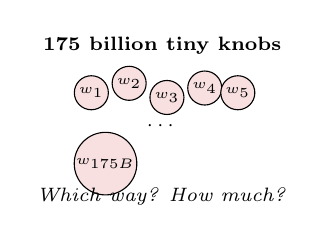
\begin{tikzpicture}[scale=0.6]
  \node[font=\scriptsize] at (0,3.5) {\textbf{175 billion tiny knobs}};
  \node[draw, circle, fill=calculusRed!15, inner sep=1pt, font=\tiny] at (-1.5,2.5) {$w_1$};
  \node[draw, circle, fill=calculusRed!15, inner sep=1pt, font=\tiny] at (-0.7,2.7) {$w_2$};
  \node[draw, circle, fill=calculusRed!15, inner sep=1pt, font=\tiny] at (0.1,2.4) {$w_3$};
  \node[draw, circle, fill=calculusRed!15, inner sep=1pt, font=\tiny] at (0.9,2.6) {$w_4$};
  \node[draw, circle, fill=calculusRed!15, inner sep=1pt, font=\tiny] at (1.6,2.5) {$w_5$};
  \node[font=\scriptsize] at (0,1.8) {$\cdots$};
  \node[draw, circle, fill=calculusRed!15, inner sep=0.5pt, font=\tiny] at (-1.2,1.0) {$w_{175B}$};
  \node[font=\scriptsize] at (0,0.3) {\textit{Which way? How much?}};
\end{tikzpicture}
\end{center}
\end{columns}

\note{
``The AI said `dog.' That is wrong. Cross-entropy says the loss is high. Now the AI needs to adjust its parameters -- all 175 billion of them -- so that next time, `mat' gets a higher score and `dog' gets a lower score.

But you cannot just randomly wiggle 175 billion knobs. You need a systematic way to know WHICH direction to adjust EACH one. That is calculus.''
}
\end{frame}

% ============================================================
% SLIDE 14: The History -- Cauchy and Gradient Descent
% ============================================================
\begin{frame}{Gradient Descent: Compute the Slope, Step Downhill, Repeat}

\begin{columns}[T]
\column{0.48\textwidth}
\textbf{Cauchy, 1847 (Paris):}\\[4pt]
If you can compute the \textbf{slope} at any point, you can find the bottom by always stepping \textbf{downhill}.

\vspace{0.5em}
\textbf{The Recipe:}
\begin{enumerate}\small
  \item Where am I? {\scriptsize(current loss)}
  \item Which way is downhill? {\scriptsize(derivative)}
  \item Take a step. {\scriptsize(learning rate $\times$ gradient)}
  \item Repeat. {\scriptsize(billions of times)}
\end{enumerate}

\vspace{0.3em}
{\small Newton \& Leibniz (1680s) gave us the derivative. Cauchy gave us the \textbf{algorithm}.}

\column{0.48\textwidth}
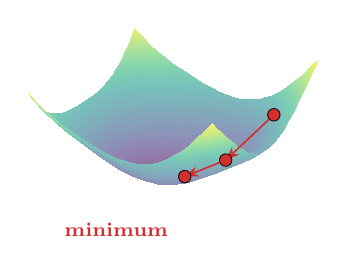
\begin{tikzpicture}[scale=0.75]
\begin{axis}[
    width=6.5cm, height=5.5cm,
    axis lines=none,
    view={30}{30},
    colormap/viridis,
    samples=25,
]
\addplot3[surf, opacity=0.6, shader=interp, domain=-2:2, y domain=-2:2]
    {x^2 + y^2 + 0.5*sin(deg(2*x))*cos(deg(2*y))};
% Ball markers
\addplot3[only marks, mark=*, mark size=3pt, fill=calculusRed]
    coordinates {(1.5,1.2,4.5) (0.8,0.6,1.2) (0.2,0.1,0.1)};
\draw[-Stealth, thick, calculusRed] (axis cs:1.5,1.2,4.5) -- (axis cs:0.8,0.6,1.2);
\draw[-Stealth, thick, calculusRed] (axis cs:0.8,0.6,1.2) -- (axis cs:0.2,0.1,0.1);
\end{axis}
\node[font=\scriptsize, calculusRed] at (1.5,0.2) {\textbf{minimum}};
\end{tikzpicture}
\end{columns}

\note{
``Archimedes was doing proto-calculus in 250 BCE. Newton and Leibniz formalized the derivative in the 1680s. But the hero for AI is Cauchy.

In 1847 he asked: if I can compute the slope at any point, can I find the bottom of a valley by always stepping downhill? Yes. That is gradient descent.

Every AI on Earth learns this way: compute the slope, step downhill, repeat. Billions of times.''

Bridge: ``Cauchy found the valley floor. But how does the slope information travel BACKWARD through 96 layers?''
}
\end{frame}

% ============================================================
% SLIDE 15: The Mechanism -- Backpropagation and the Chain Rule
% ============================================================
\begin{frame}{The Chain Rule Trains Every AI}

\begin{columns}[T]
\column{0.48\textwidth}
\textbf{The chain rule:}\\[2pt]
\vspace{-0.4em}
$$\frac{d}{dx}f(g(x)) = f'(g(x))\cdot g'(x)$$

\vspace{0.1em}
{\small Derivative of a composition = product of individual derivatives.}

\vspace{0.3em}
\textbf{In a network:}\\[2pt]
{\small Error flows \textbf{backward}, layer by layer. Each layer learns its contribution to the mistake.}

\vspace{0.3em}
{\small\begin{tabular}{ll}
\textbf{1970} & Linnainmaa: auto-differentiation \\
\textbf{1986} & \raisebox{-0.2cm}{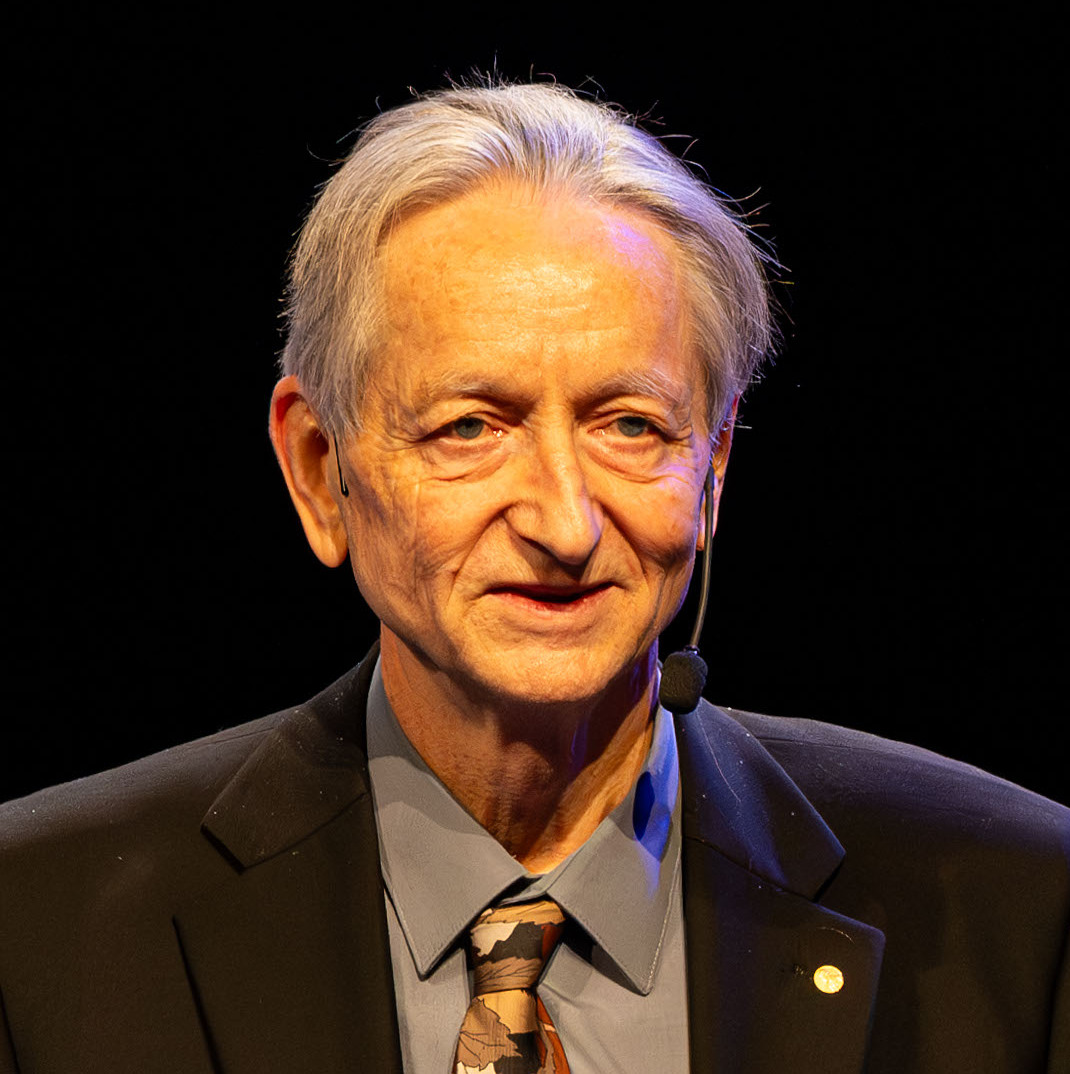
\includegraphics[height=0.6cm]{figures/hinton.jpg}} Hinton: backprop\\
\end{tabular}}

\column{0.48\textwidth}
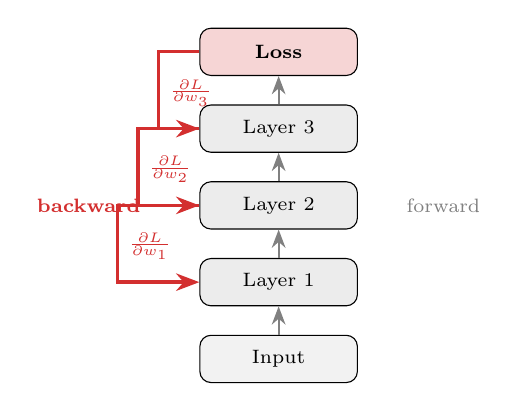
\begin{tikzpicture}[scale=0.65, every node/.style={font=\scriptsize}]
  % Forward pass (left)
  \node[draw, rounded corners, fill=gray!10, minimum width=2cm, minimum height=0.6cm]
    (in) at (0,0) {Input};
  \node[draw, rounded corners, fill=gray!15, minimum width=2cm, minimum height=0.6cm]
    (l1) at (0,1.5) {Layer 1};
  \node[draw, rounded corners, fill=gray!15, minimum width=2cm, minimum height=0.6cm]
    (l2) at (0,3.0) {Layer 2};
  \node[draw, rounded corners, fill=gray!15, minimum width=2cm, minimum height=0.6cm]
    (l3) at (0,4.5) {Layer 3};
  \node[draw, rounded corners, fill=calculusRed!20, minimum width=2cm, minimum height=0.6cm]
    (loss) at (0,6.0) {\textbf{Loss}};
  % Forward arrows
  \draw[-Stealth, thick, gray] (in) -- (l1);
  \draw[-Stealth, thick, gray] (l1) -- (l2);
  \draw[-Stealth, thick, gray] (l2) -- (l3);
  \draw[-Stealth, thick, gray] (l3) -- (loss);
  % Backward arrows
  \draw[-Stealth, very thick, calculusRed] (loss.west) -- +(-0.8,0) |- (l3.west);
  \draw[-Stealth, very thick, calculusRed] (l3.west) -- +(-1.2,0) |- (l2.west);
  \draw[-Stealth, very thick, calculusRed] (l2.west) -- +(-1.6,0) |- (l1.west);
  % Labels
  \node[right=0.2cm, gray, font=\scriptsize] at (2.0,3.0) {forward};
  \node[left=0.2cm, calculusRed, font=\scriptsize\bfseries] at (-2.2,3.0) {backward};
  \node[left=0.2cm, calculusRed, font=\tiny] at (-0.8,5.2) {$\frac{\partial L}{\partial w_3}$};
  \node[left=0.2cm, calculusRed, font=\tiny] at (-1.2,3.7) {$\frac{\partial L}{\partial w_2}$};
  \node[left=0.2cm, calculusRed, font=\tiny] at (-1.6,2.2) {$\frac{\partial L}{\partial w_1}$};
\end{tikzpicture}
\end{columns}

\note{
``The chain rule from your calculus class: the derivative of a composition is the product of the individual derivatives.

Linnainmaa automated this in 1970. Hinton made it famous for neural networks in 1986.

The algorithm: compute the loss at the output, then send the error signal backward, layer by layer, using the chain rule. Each layer learns how much it contributed to the error and adjusts accordingly.

This is how 175 billion parameters learn from one wrong prediction.''
}
\end{frame}

% ============================================================
% SLIDE 16: The Mechanism -- The Training Loop
% ============================================================
\begin{frame}{The Training Loop}

\begin{center}
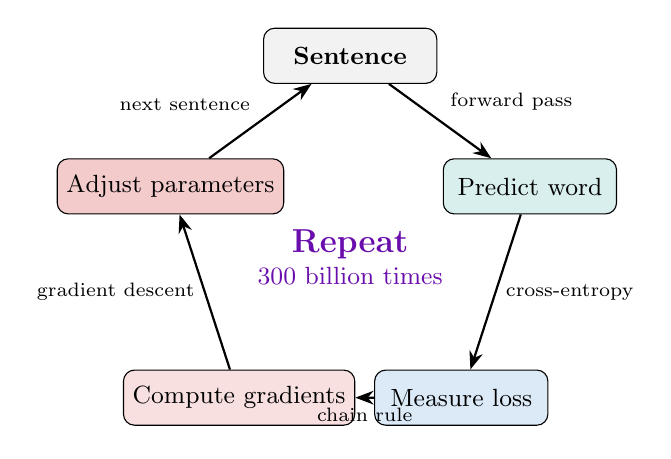
\begin{tikzpicture}[scale=0.80, every node/.style={font=\small}]
  % Circular training loop
  \node[draw, fill=gray!10, rounded corners, minimum width=2.2cm, minimum height=0.7cm]
    (sent) at (90:3) {\textbf{Sentence}};
  \node[draw, fill=linalgTeal!15, rounded corners, minimum width=2.2cm, minimum height=0.7cm]
    (pred) at (18:3) {Predict word};
  \node[draw, fill=probBlue!15, rounded corners, minimum width=2.2cm, minimum height=0.7cm]
    (loss) at (-54:3) {Measure loss};
  \node[draw, fill=calculusRed!15, rounded corners, minimum width=2.2cm, minimum height=0.7cm]
    (grad) at (-126:3) {Compute gradients};
  \node[draw, fill=calculusRed!25, rounded corners, minimum width=2.2cm, minimum height=0.7cm]
    (adj) at (-198:3) {Adjust parameters};
  % Arrows
  \draw[-Stealth, thick] (sent) -- (pred) node[midway, above right, font=\scriptsize] {forward pass};
  \draw[-Stealth, thick] (pred) -- (loss) node[midway, right, font=\scriptsize] {cross-entropy};
  \draw[-Stealth, thick] (loss) -- (grad) node[midway, below, font=\scriptsize] {chain rule};
  \draw[-Stealth, thick] (grad) -- (adj) node[midway, left, font=\scriptsize] {gradient descent};
  \draw[-Stealth, thick] (adj) -- (sent) node[midway, above left, font=\scriptsize] {next sentence};
  % Center label
  \node[font=\large\bfseries, aiViolet] at (0,0) {Repeat};
  \node[font=\small, aiViolet] at (0,-0.5) {300 billion times};
\end{tikzpicture}
\end{center}

\vspace{-0.3em}

\begin{insightbox}
\small GPT-3 ran this loop on 300 billion tokens. Same math every time: Topics 1 + 2 + 3.
\end{insightbox}

\note{
``The full loop: read a sentence, predict the next word, measure the loss with Shannon's cross-entropy, compute the gradients with the chain rule, adjust the parameters with Cauchy's gradient descent, move to the next sentence.

GPT-3 did this loop 300 billion times. The same math, the same loop, 300 billion repetitions.''

Bridge: ``The AI can now learn. But there is a problem: `The cat sat on the mat because it was tired.' What does `it' refer to?''
}
\end{frame}

% ============================================================
% SLIDE 17: Inside the LLM -- Where Calculus Lives
% ============================================================
\begin{frame}{Building Block Found: Derivatives, Gradient Descent, Backpropagation}

\begin{columns}[T]
\column{0.55\textwidth}
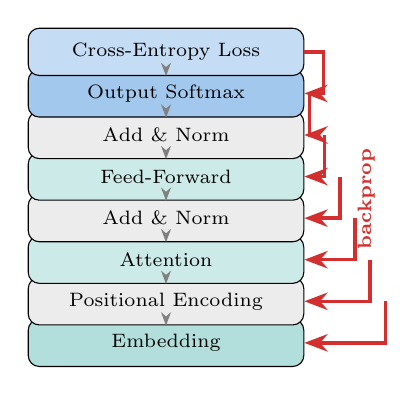
\begin{tikzpicture}[scale=0.48, every node/.style={font=\scriptsize}]
  \node[draw, fill=linalgTeal!30, rounded corners, minimum width=3.5cm, minimum height=0.6cm]
    (emb) at (0,0) {Embedding};
  \node[draw, fill=gray!15, rounded corners, minimum width=3.5cm, minimum height=0.6cm]
    (pos) at (0,1.1) {Positional Encoding};
  \node[draw, fill=linalgTeal!20, rounded corners, minimum width=3.5cm, minimum height=0.6cm]
    (attn) at (0,2.2) {Attention};
  \node[draw, fill=gray!15, rounded corners, minimum width=3.5cm, minimum height=0.6cm]
    (an1) at (0,3.3) {Add \& Norm};
  \node[draw, fill=linalgTeal!20, rounded corners, minimum width=3.5cm, minimum height=0.6cm]
    (ff) at (0,4.4) {Feed-Forward};
  \node[draw, fill=gray!15, rounded corners, minimum width=3.5cm, minimum height=0.6cm]
    (an2) at (0,5.5) {Add \& Norm};
  \node[draw, fill=probBlue!40, rounded corners, minimum width=3.5cm, minimum height=0.6cm]
    (out) at (0,6.6) {Output Softmax};
  \node[draw, fill=probBlue!25, rounded corners, minimum width=3.5cm, minimum height=0.6cm]
    (loss) at (0,7.7) {Cross-Entropy Loss};
  % Forward
  \draw[-Stealth, gray] (emb) -- (pos);
  \draw[-Stealth, gray] (pos) -- (attn);
  \draw[-Stealth, gray] (attn) -- (an1);
  \draw[-Stealth, gray] (an1) -- (ff);
  \draw[-Stealth, gray] (ff) -- (an2);
  \draw[-Stealth, gray] (an2) -- (out);
  \draw[-Stealth, gray] (out) -- (loss);
  % Backward arrows
  \draw[-Stealth, very thick, calculusRed] (loss.east) -- +(0.5,0) |- (out.east);
  \draw[-Stealth, very thick, calculusRed] (3.8,6.6) |- (an2.east);
  \draw[-Stealth, very thick, calculusRed] (4.2,5.5) |- (ff.east);
  \draw[-Stealth, very thick, calculusRed] (4.6,4.4) |- (an1.east);
  \draw[-Stealth, very thick, calculusRed] (5.0,3.3) |- (attn.east);
  \draw[-Stealth, very thick, calculusRed] (5.4,2.2) |- (pos.east);
  \draw[-Stealth, very thick, calculusRed] (5.8,1.1) |- (emb.east);
  \node[calculusRed, font=\scriptsize\bfseries, rotate=90] at (5.3,3.8) {backprop};
\end{tikzpicture}

\column{0.42\textwidth}
\textbf{Where Topic 3 lives:}
\begin{itemize}\small
  \item \textcolor{calculusRed}{\textbf{Backward pass}} -- gradient descent (Cauchy, 1847)
  \item \textcolor{calculusRed}{\textbf{Chain rule}} -- error flows through layers (Linnainmaa / Hinton)
\end{itemize}

\vspace{0.4em}
\progressbar{3}

\vspace{0.2em}
\begin{center}
\small\textit{The AI can represent, predict, and learn. But it has no notion of \textbf{context}.}
\end{center}
\end{columns}

\note{
``The forward pass uses linear algebra and probability. The backward pass uses calculus. Every arrow flowing backward through the transformer is the chain rule in action.

Cauchy's gradient descent, Linnainmaa's automatic differentiation, Hinton's backpropagation. Three building blocks found.''

Bridge: ``The AI can represent words, predict, and learn. But it still processes words one at a time. It has no notion of CONTEXT.''
}
\end{frame}

% ============================================================
% TOPIC 4: How does it understand context?
% Color: seqIndigo  |  Slides 18--23
% ============================================================

% ============================================================
% SLIDE 18: The Question -- The Problem of "It"
% ============================================================
\begin{frame}{``The cat sat on the mat because IT was \rule{1cm}{0.4pt}'' -- What Does ``It'' Mean?}

\topicquestion{seqIndigo}{The word ``it'' could mean ``cat'' or ``mat.'' The AI needs to look at the WHOLE sentence to decide. How?}

\vspace{0.3em}

\begin{center}
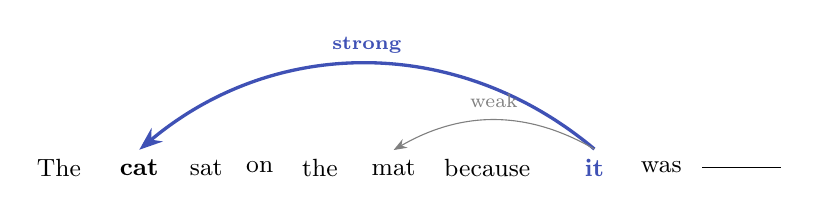
\begin{tikzpicture}[scale=0.85, every node/.style={font=\small}]
  % Words
  \node (the1) at (0,0) {The};
  \node (cat) at (1.2,0) {\textbf{cat}};
  \node (sat) at (2.2,0) {sat};
  \node (on) at (3.0,0) {on};
  \node (the2) at (3.9,0) {the};
  \node (mat) at (5.0,0) {mat};
  \node (bec) at (6.4,0) {because};
  \node[seqIndigo, font=\bfseries\small] (it) at (8.0,0) {it};
  \node (was) at (9.0,0) {was};
  \node (tired) at (10.2,0) {\rule{1cm}{0.3pt}};
  % Attention arrows
  \draw[-Stealth, very thick, seqIndigo] (it.north) to[out=140, in=40] node[midway, above, font=\scriptsize\bfseries] {strong} (cat.north);
  \draw[-Stealth, thin, gray] (it.north) to[out=150, in=30] (mat.north);
  \node[gray, font=\scriptsize] at (6.5,1.0) {weak};
\end{tikzpicture}
\end{center}

\vspace{0.2em}

\begin{center}
\small Before 2014, AI processed words one at a time. Early words were \textbf{forgotten} after $\sim$50 words.
\end{center}

\note{
``Here is a problem the first three topics cannot solve. `The cat sat on the mat because it was tired.' You know `it' means `cat.' But how? Because you understand context -- you looked back at the whole sentence.

Before 2014, AI could not do this well. Words were processed one at a time, and early words were forgotten.''

This is the fourth facet of ``predicting the next word.''
}
\end{frame}

% ============================================================
% SLIDE 19: The History -- Markov, Bahdanau, Vaswani
% ============================================================
\begin{frame}{From Poetry Analysis to ``Attention Is All You Need''}

\begin{columns}[T]
\column{0.32\textwidth}
\begin{tcolorbox}[colframe=seqIndigo, colback=seqIndigo!5, boxrule=1pt,
  fonttitle=\bfseries\small, title={Markov, 1906}, left=2pt, right=2pt, top=2pt, bottom=2pt]
\centering\small
Analyzed Pushkin's poetry.\\[2pt]
\textbf{Markov chains}: next state depends on current state.\\[2pt]
But chains \textbf{forget}.
\end{tcolorbox}

\column{0.32\textwidth}
\begin{tcolorbox}[colframe=seqIndigo, colback=seqIndigo!5, boxrule=1pt,
  fonttitle=\bfseries\small, title={Bahdanau, 2014}, left=2pt, right=2pt, top=2pt, bottom=2pt]
\centering\small
Montreal. Translation.\\[2pt]
``Why compress into one vector?\\[2pt]
\textbf{Look back} at the whole input.''\\[2pt]
Invented \textbf{attention}.
\end{tcolorbox}

\column{0.32\textwidth}
\begin{tcolorbox}[colframe=seqIndigo, colback=seqIndigo!5, boxrule=1pt,
  fonttitle=\bfseries\small, title={Vaswani et al., 2017}, left=2pt, right=2pt, top=2pt, bottom=2pt]
\centering\small
Google. 8 authors.\\[2pt]
``\textbf{Attention Is All You Need}''\\[2pt]
Architecture using \textbf{only} attention.\\[2pt]
The \textbf{transformer}.
\end{tcolorbox}
\end{columns}

\vspace{0.2em}
\begin{insightbox}
\small Markov started it. Bahdanau cracked the memory problem. Vaswani assembled the machine.
\end{insightbox}

\note{
``Markov analyzed Russian poetry to prove a point about probability. His chain model became the ancestor of every language model. But Markov chains forget. RNNs forget. After 50 words, the beginning is gone.

Then in 2014, Bahdanau asked: why compress everything into one vector when you can look back at the whole input? That is attention.

Three years later, Vaswani and seven colleagues built an entire architecture using ONLY attention. They called the paper `Attention Is All You Need.' They were right.''
}
\end{frame}

% ============================================================
% SLIDE 20: The Mechanism -- Self-Attention
% ============================================================
\begin{frame}{Every Word Looks at Every Other Word}

\begin{columns}[T]
\column{0.52\textwidth}
\textbf{Self-Attention: Q, K, V}
\begin{itemize}\small
  \item \textbf{Q}uery: ``What am I looking for?''
  \item \textbf{K}ey: ``What do I contain?''
  \item \textbf{V}alue: ``What information do I carry?''
\end{itemize}

\vspace{0.2em}
{\small Attention score = dot product of Q and K (Gibbs, T1!)\\
Then softmax turns scores into weights (Boltzmann, T2!)}

\vspace{0.3em}
$$\text{Attention}(Q,K,V) = \text{softmax}\!\left(\frac{QK^\top}{\sqrt{d}}\right) V$$

\column{0.44\textwidth}
\vspace{-0.3em}
{\small\textbf{Attention heatmap:}}

\vspace{0.2em}
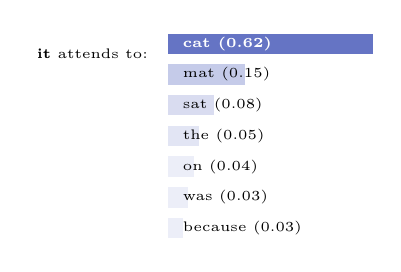
\begin{tikzpicture}[scale=0.65, every node/.style={font=\tiny}]
  % Heatmap for "it"
  \node[anchor=east] at (-0.2,0) {\textbf{it} attends to:};
  % Bars
  \fill[seqIndigo!80] (0,0) rectangle (4.0,0.4);
  \node[right, white, font=\tiny\bfseries] at (0.1,0.2) {cat (0.62)};
  \fill[seqIndigo!30] (0,-0.6) rectangle (1.5,-0.2);
  \node[right, font=\tiny] at (0.1,-0.4) {mat (0.15)};
  \fill[seqIndigo!20] (0,-1.2) rectangle (0.9,-0.8);
  \node[right, font=\tiny] at (0.1,-1.0) {sat (0.08)};
  \fill[seqIndigo!15] (0,-1.8) rectangle (0.6,-1.4);
  \node[right, font=\tiny] at (0.1,-1.6) {the (0.05)};
  \fill[seqIndigo!10] (0,-2.4) rectangle (0.5,-2.0);
  \node[right, font=\tiny] at (0.1,-2.2) {on (0.04)};
  \fill[seqIndigo!10] (0,-3.0) rectangle (0.4,-2.6);
  \node[right, font=\tiny] at (0.1,-2.8) {was (0.03)};
  \fill[seqIndigo!10] (0,-3.6) rectangle (0.3,-3.2);
  \node[right, font=\tiny] at (0.1,-3.4) {because (0.03)};
\end{tikzpicture}

\vspace{0.3em}
{\scriptsize``it'' looks back at ``cat'' and assigns high weight. Context resolved.}
\end{columns}

\note{
``Each word asks a question (Q). Each word offers a key (K). Self-attention computes the dot product -- that is Gibbs, from Topic 1 -- between every Q and every K.

`It' asks: `What am I referring to?' `Cat' answers: `I am an animate noun.' Their dot product is high.

Then the softmax -- Boltzmann, from Topic 2 -- turns these scores into attention weights. The word `it' now knows it means `cat.'

One equation, and it uses the dot product, softmax, and matrix multiplication you already learned.''
}
\end{frame}

% ============================================================
% SLIDE 21: The Mechanism -- Positional Encoding and the Full Layer
% ============================================================
\begin{frame}{Fourier's Sine Waves Tell the AI Where Each Word Is}

\begin{columns}[T]
\column{0.48\textwidth}
\textbf{The problem:} Self-attention has no sense of word \textbf{order}.

\vspace{0.3em}
\textbf{The solution:} Positional encoding using sine and cosine waves at different frequencies.

\vspace{0.2em}
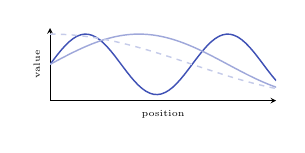
\begin{tikzpicture}[scale=0.65]
\begin{axis}[
    width=6cm, height=3cm,
    axis lines=left, xlabel={\tiny position}, ylabel={\tiny value},
    xmin=0, xmax=20, ymin=-1.2, ymax=1.2,
    xtick=\empty, ytick=\empty,
    no markers
]
\addplot[domain=0:20, samples=60, thick, seqIndigo] {sin(deg(x/2))};
\addplot[domain=0:20, samples=60, thick, seqIndigo!50] {sin(deg(x/5))};
\addplot[domain=0:20, samples=60, thick, seqIndigo!30, dashed] {cos(deg(x/8))};
\end{axis}
\end{tikzpicture}

\vspace{0.1em}
{\small\textbf{Fourier, 1807}: decomposed heat into waves.\\
\textbf{Vaswani, 2017}: decomposed position into waves.\\
Same math, 210 years apart.}

\column{0.48\textwidth}
\textbf{One Transformer Layer:}

\vspace{0.3em}
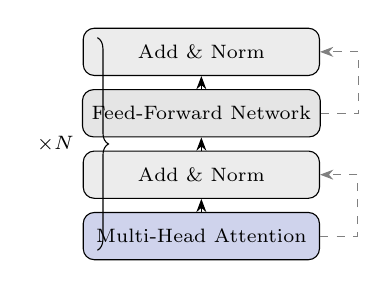
\begin{tikzpicture}[scale=0.60, every node/.style={font=\scriptsize}]
  \node[draw, fill=seqIndigo!25, rounded corners, minimum width=3cm, minimum height=0.6cm]
    (mha) at (0,0) {Multi-Head Attention};
  \node[draw, fill=gray!15, rounded corners, minimum width=3cm, minimum height=0.6cm]
    (an1) at (0,1.3) {Add \& Norm};
  \node[draw, fill=gray!20, rounded corners, minimum width=3cm, minimum height=0.6cm]
    (ffn) at (0,2.6) {Feed-Forward Network};
  \node[draw, fill=gray!15, rounded corners, minimum width=3cm, minimum height=0.6cm]
    (an2) at (0,3.9) {Add \& Norm};
  % Arrows
  \draw[-Stealth] (mha) -- (an1);
  \draw[-Stealth] (an1) -- (ffn);
  \draw[-Stealth] (ffn) -- (an2);
  % Skip connections
  \draw[-Stealth, dashed, gray] (mha.east) -- +(0.8,0) |- (an1.east);
  \draw[-Stealth, dashed, gray] (ffn.east) -- +(0.8,0) |- (an2.east);
  % Brace
  \draw[decorate, decoration={brace, amplitude=4pt, mirror}] (-2.2,-0.3) -- (-2.2,4.2)
    node[midway, left=5pt, font=\scriptsize] {$\times N$};
\end{tikzpicture}

\vspace{0.2em}
{\small Stack $N=96$ of these $\rightarrow$ GPT-4.}
\end{columns}

\note{
``The transformer has no built-in sense of word order. To fix this, Vaswani added positional encodings -- sine and cosine functions at different frequencies. This is Fourier's idea from 1807.

One transformer layer: self-attention (Bahdanau/Vaswani), then a feed-forward network, with two rounds of `add and normalize.'

Stack 96 of these and you have GPT-4.''
}
\end{frame}

% ============================================================
% SLIDE 22: THE CLIMAX -- The Full Annotated Transformer
% ============================================================
\begin{frame}{2,000 Years of Mathematics in One Diagram}

\vspace{-0.7em}
\begin{center}
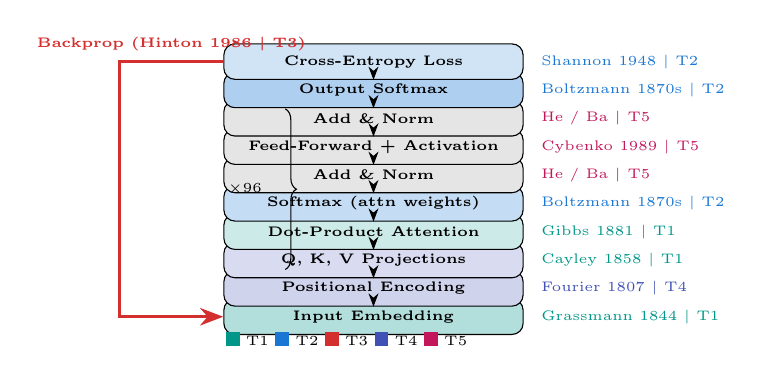
\begin{tikzpicture}[scale=0.40, every node/.style={font=\tiny}]
  \node[draw, fill=linalgTeal!30, rounded corners, minimum width=3.8cm, minimum height=0.45cm]
    (emb) at (0,0) {\textbf{Input Embedding}};
  \node[right=0.1cm, linalgTeal] at (emb.east) {Grassmann 1844 \textbar{} T1};

  \node[draw, fill=seqIndigo!25, rounded corners, minimum width=3.8cm, minimum height=0.45cm]
    (pos) at (0,0.9) {\textbf{Positional Encoding}};
  \node[right=0.1cm, seqIndigo] at (pos.east) {Fourier 1807 \textbar{} T4};

  \node[draw, fill=seqIndigo!20, rounded corners, minimum width=3.8cm, minimum height=0.45cm]
    (qkv) at (0,1.8) {\textbf{Q, K, V Projections}};
  \node[right=0.1cm, linalgTeal] at (qkv.east) {Cayley 1858 \textbar{} T1};

  \node[draw, fill=linalgTeal!20, rounded corners, minimum width=3.8cm, minimum height=0.45cm]
    (dot) at (0,2.7) {\textbf{Dot-Product Attention}};
  \node[right=0.1cm, linalgTeal] at (dot.east) {Gibbs 1881 \textbar{} T1};

  \node[draw, fill=probBlue!25, rounded corners, minimum width=3.8cm, minimum height=0.45cm]
    (sm1) at (0,3.6) {\textbf{Softmax (attn weights)}};
  \node[right=0.1cm, probBlue] at (sm1.east) {Boltzmann 1870s \textbar{} T2};

  \node[draw, fill=gray!20, rounded corners, minimum width=3.8cm, minimum height=0.45cm]
    (an1) at (0,4.5) {\textbf{Add \& Norm}};
  \node[right=0.1cm, neuronPink] at (an1.east) {He / Ba \textbar{} T5};

  \node[draw, fill=gray!20, rounded corners, minimum width=3.8cm, minimum height=0.45cm]
    (ffn) at (0,5.4) {\textbf{Feed-Forward + Activation}};
  \node[right=0.1cm, neuronPink] at (ffn.east) {Cybenko 1989 \textbar{} T5};

  \node[draw, fill=gray!20, rounded corners, minimum width=3.8cm, minimum height=0.45cm]
    (an2) at (0,6.3) {\textbf{Add \& Norm}};
  \node[right=0.1cm, neuronPink] at (an2.east) {He / Ba \textbar{} T5};

  \node[draw, fill=probBlue!35, rounded corners, minimum width=3.8cm, minimum height=0.45cm]
    (outsm) at (0,7.2) {\textbf{Output Softmax}};
  \node[right=0.1cm, probBlue] at (outsm.east) {Boltzmann 1870s \textbar{} T2};

  \draw[-Stealth] (emb) -- (pos);
  \draw[-Stealth] (pos) -- (qkv);
  \draw[-Stealth] (qkv) -- (dot);
  \draw[-Stealth] (dot) -- (sm1);
  \draw[-Stealth] (sm1) -- (an1);
  \draw[-Stealth] (an1) -- (ffn);
  \draw[-Stealth] (ffn) -- (an2);
  \draw[-Stealth] (an2) -- (outsm);

  \draw[decorate, decoration={brace, amplitude=4pt, mirror}] (-2.8,1.5) -- (-2.8,6.6)
    node[midway, left=5pt, font=\tiny\bfseries] {$\times 96$};

  \node[draw, fill=probBlue!20, rounded corners, minimum width=3.8cm, minimum height=0.45cm]
    (ce) at (0,8.1) {\textbf{Cross-Entropy Loss}};
  \node[right=0.1cm, probBlue] at (ce.east) {Shannon 1948 \textbar{} T2};
  \draw[-Stealth] (outsm) -- (ce);

  \draw[-Stealth, very thick, calculusRed] (ce.west) -- +(-3.3,0)
    node[midway, above, font=\tiny\bfseries, calculusRed] {Backprop (Hinton 1986 \textbar{} T3)} |- (emb.west);

  \node[font=\tiny, anchor=west] at (-5.0,-0.7) {%
    \textcolor{linalgTeal}{\rule{5pt}{5pt}} T1
    \textcolor{probBlue}{\rule{5pt}{5pt}} T2
    \textcolor{calculusRed}{\rule{5pt}{5pt}} T3
    \textcolor{seqIndigo}{\rule{5pt}{5pt}} T4
    \textcolor{neuronPink}{\rule{5pt}{5pt}} T5};
\end{tikzpicture}
\end{center}

\note{
[PAUSE. Let the diagram land.]

``Every single piece has a name, a date, and a topic where you learned it. The sine functions come from Fourier in 1807. The dot products from Gibbs in 1881. The softmax from Boltzmann in the 1870s.

The training uses Cauchy's gradient descent from 1847 and Hinton's backpropagation from 1986.

When you talk to an AI, you are talking to 2,000 years of mathematics, all running at once.''

Bridge: ``This is the FULL machine that predicts `mat' from `The cat sat on the blank.' But two components are labeled `Topic 5.' We have not explained those yet.''
}
\end{frame}

% ============================================================
% SLIDE 23: Inside the LLM -- Where Context Lives
% ============================================================
\begin{frame}{Building Block Found: Attention, Self-Attention, Positional Encoding}

\begin{columns}[T]
\column{0.55\textwidth}
\textbf{The transformer IS Topics 1--4 combined:}

\vspace{0.3em}
\begin{itemize}\small
  \item \textcolor{linalgTeal}{\textbf{T1}}: Embeddings, dot products, matrix mult
  \item \textcolor{probBlue}{\textbf{T2}}: Softmax, cross-entropy
  \item \textcolor{calculusRed}{\textbf{T3}}: Backpropagation, gradient descent
  \item \textcolor{seqIndigo}{\textbf{T4}}: Attention, position, the architecture
\end{itemize}

\vspace{0.3em}
{\small Vaswani et al.\ (2017): 8 authors assembled 2,000 years of math into one architecture.}

\column{0.42\textwidth}
\progressbar{4}

\vspace{0.3em}
{\small\textbf{The five questions:}}\\[3pt]
\textcolor{linalgTeal}{\faCheckSquare}~Similar words\\
\textcolor{probBlue}{\faCheckSquare}~Choose next word\\
\textcolor{calculusRed}{\faCheckSquare}~Learn from mistakes\\
\textcolor{seqIndigo}{\faCheckSquare}~Understand context\\
\textcolor{gray!50}{\faSquare}~Get so good\\[6pt]
{\small\textit{The machine works. But why do 96 layers work so much better than one?}}
\end{columns}

\note{
``Four of five building blocks found. The transformer is not a new invention layered on top of the others -- it IS the combination of all of them.

Attention is the dot product from Topic 1 applied to context. Softmax from Topic 2 weights the attention. Backpropagation from Topic 3 trains it. The architecture from Topic 4 wires them together.

One question remains: how does it get so good?''
}
\end{frame}

% ============================================================
% TOPIC 5: How does it get so good?
% Color: neuronPink  |  Slides 24--28
% ============================================================

% ============================================================
% SLIDE 24: The Question -- The Mystery of Scale
% ============================================================
\begin{frame}{``The cat sat on the \rule{1.2cm}{0.4pt}'' -- One Layer Is Dumb. 96 Layers Are Brilliant. Why?}

\topicquestion{neuronPink}{One layer is mediocre. 96 layers are brilliant. 175B parameters. How does scale turn simple math into something that feels like intelligence?}

\vspace{0.2em}

\begin{columns}[T]
\column{0.46\textwidth}
\textbf{1 layer predicts:}\\[4pt]
\begin{tabular}{ll}
the & 22\% \\
a & 18\% \\
was & 12\% \\
\end{tabular}\\[4pt]
{\small Vague. Generic. Useless.}

\column{0.46\textwidth}
\textbf{96 layers predict:}\\[4pt]
\begin{tabular}{ll}
mat & 68\% \\
floor & 15\% \\
table & 8\% \\
\end{tabular}\\[4pt]
{\small Precise. Contextual. Useful.}
\end{columns}

\vspace{0.3em}
\begin{center}
\small Same architecture. Same math. Just \textbf{deeper} and \textbf{bigger}. Why does that work?
\end{center}

\note{
``We have the complete machine. But there is a mystery. One layer of self-attention barely works. Stack 96 layers, add 175 billion parameters, train on 300 billion tokens -- and suddenly it writes poetry, solves math problems, and translates languages.

Same architecture. Same math. Just bigger. Why does scale work?''
}
\end{frame}

% ============================================================
% SLIDE 25: The History -- The Neuron, the Crash, the Comeback
% ============================================================
\begin{frame}{1943: Invention. \quad 1969: Crash. \quad 1986: Comeback.}

\begin{tikzpicture}[scale=0.78, every node/.style={font=\small}]
  % Timeline
  \draw[thick, gray] (0,0) -- (12,0);

  % 1943
  \fill[neuronPink] (0.5,0) circle (4pt);
  \node[above=3pt, font=\small\bfseries] at (0.5,0) {1943};
  \node[below=5pt, text width=2.5cm, align=center, font=\scriptsize] at (0.5,0)
    {McCulloch \& Pitts\\The mathematical\\neuron};

  % 1958
  \fill[neuronPink] (3.5,0) circle (4pt);
  \node[above=3pt, font=\small\bfseries] at (3.5,0) {1958};
  \node[below=5pt, text width=2.5cm, align=center, font=\scriptsize] at (3.5,0)
    {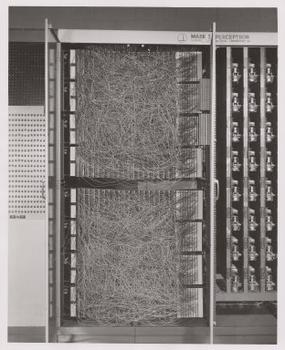
\includegraphics[height=0.8cm]{figures/perceptron.jpg}\\Rosenblatt\\``A machine that\\could think''};

  % 1969
  \fill[calculusRed] (6.5,0) circle (4pt);
  \node[above=3pt, font=\small\bfseries, calculusRed] at (6.5,0) {1969};
  \node[below=5pt, text width=2.8cm, align=center, font=\scriptsize] at (6.5,0)
    {Minsky \& Papert\\XOR: one layer\\cannot learn this.\\[1pt]\textbf{AI Winter.}};

  % 1986
  \fill[approxGreen] (9.5,0) circle (4pt);
  \node[above=3pt, font=\small\bfseries, approxGreen] at (9.5,0) {1986};
  \node[below=5pt, text width=2.5cm, align=center, font=\scriptsize] at (9.5,0)
    {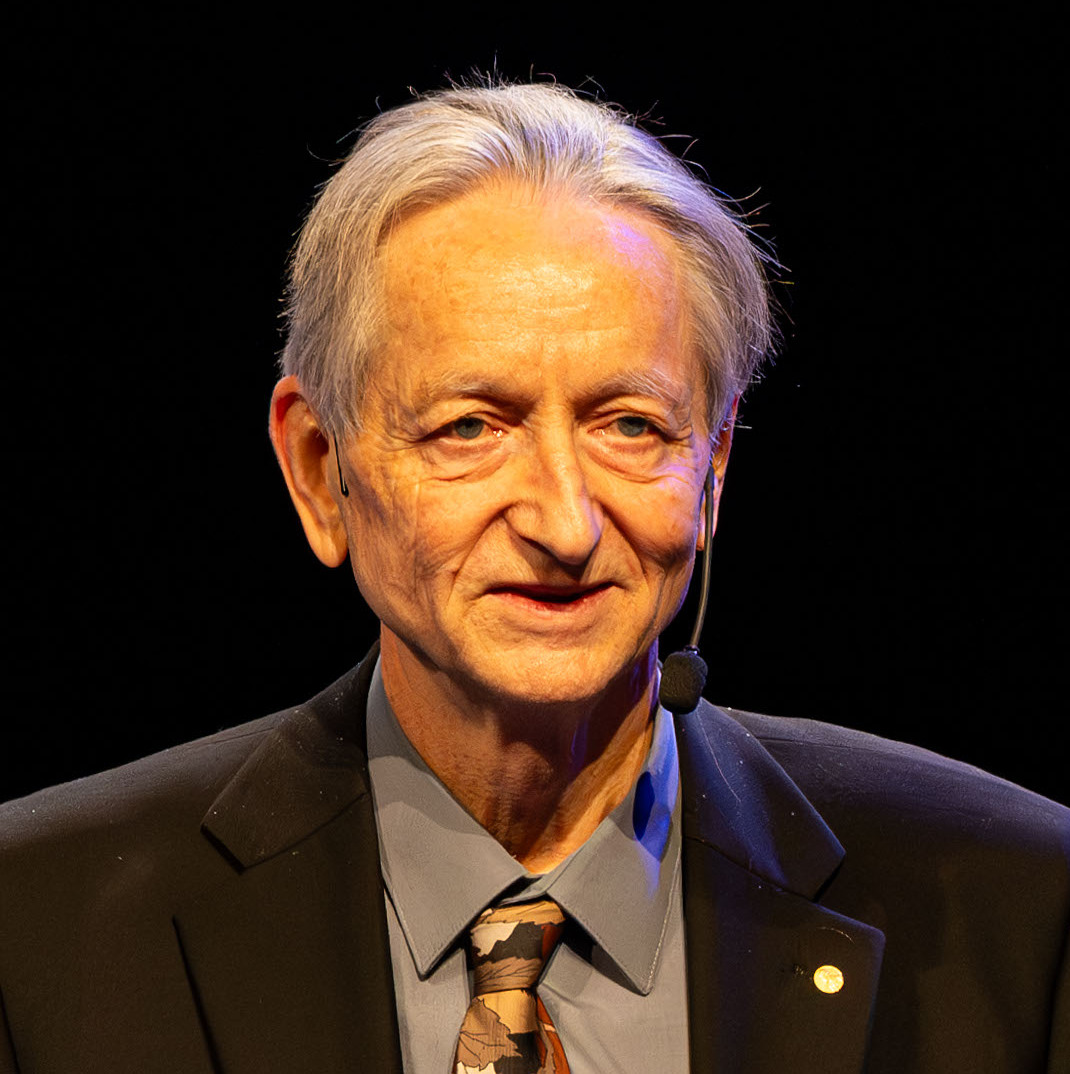
\includegraphics[height=0.8cm]{figures/hinton.jpg}\\Hinton\\Backprop (Topic~3!)\\revives deep nets};

  % Drama arc
  \draw[thick, neuronPink, -{Stealth}] (0.5,1.3) -- (3.5,2.2) node[midway, above, font=\scriptsize, sloped] {hype};
  \draw[thick, calculusRed, -{Stealth}] (3.5,2.2) -- (6.5,0.5) node[midway, above, font=\scriptsize, sloped] {crash};
  \draw[thick, approxGreen, -{Stealth}] (6.5,0.5) -- (9.5,1.8) node[midway, above, font=\scriptsize, sloped] {comeback};
\end{tikzpicture}

\vspace{0.1em}
\begin{insightbox}
\small The solution: \textbf{add more layers}. But nobody knew how to train them until Hinton showed the chain rule (Topic~3) could do it.
\end{insightbox}

\note{
``McCulloch was a neurophysiologist. Pitts was about 20, self-taught, no degree. Their 1943 paper defined the mathematical neuron.

Rosenblatt built the Perceptron -- the press said it would think like a human.

Then Minsky and Papert proved that a single-layer perceptron cannot learn XOR -- a simple logic function. The field collapsed for 17 years. The AI winter.

The solution: add more layers. But nobody knew how to train multiple layers until Hinton showed that backpropagation could do it.''

Bridge: ``Multiple layers work. But 96 layers? That needed three more inventions.''
}
\end{frame}

% ============================================================
% SLIDE 26: The Mechanism -- Depth, Activation, Residuals, Normalization
% ============================================================
\begin{frame}{Three Tricks That Made Deep Networks Possible}

\begin{columns}[T]
\column{0.32\textwidth}
\begin{tcolorbox}[colframe=neuronPink, colback=neuronPink!5, boxrule=0.8pt,
  fonttitle=\bfseries\scriptsize, title={Activation}, left=2pt, right=2pt, top=1pt, bottom=1pt]
\centering\scriptsize
Without it, 96 layers = 1 layer.\\[1pt]
\textbf{Nonlinearity} matters.\\[1pt]
\begin{tikzpicture}[scale=0.30]
\begin{axis}[
  width=3cm, height=1.6cm,
  axis lines=middle, xtick=\empty, ytick=\empty,
  xmin=-3, xmax=3, ymin=-0.5, ymax=3,
  no markers
]
\addplot[domain=-3:0, samples=15, thick, neuronPink] {0};
\addplot[domain=0:3, samples=15, thick, neuronPink] {x};
\end{axis}
\end{tikzpicture}\\[-3pt]
{\scriptsize ReLU: $\max(0, x)$}
\end{tcolorbox}

\column{0.32\textwidth}
\begin{tcolorbox}[colframe=neuronPink, colback=neuronPink!5, boxrule=0.8pt,
  fonttitle=\bfseries\scriptsize, title={Residual (He, 2015)}, left=2pt, right=2pt, top=1pt, bottom=1pt]
\centering\scriptsize
Signal fades through layers.\\[1pt]
\textbf{Skip connections} fix it.\\[1pt]
$\text{out} = x + f(x)$\\[2pt]
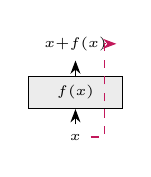
\begin{tikzpicture}[scale=0.35, every node/.style={font=\tiny}]
  \node[draw, fill=gray!15, minimum width=1.2cm] (f) at (0,0) {$f(x)$};
  \node[below=0.3cm] (in) at (0,-0.3) {$x$};
  \node[above=0.3cm] (out) at (0,0.3) {$x{+}f(x)$};
  \draw[-Stealth] (in) -- (f);
  \draw[-Stealth] (f) -- (out);
  \draw[-Stealth, dashed, neuronPink] (in.east) -- +(0.5,0) |- (out.east);
\end{tikzpicture}
\end{tcolorbox}

\column{0.32\textwidth}
\begin{tcolorbox}[colframe=neuronPink, colback=neuronPink!5, boxrule=0.8pt,
  fonttitle=\bfseries\scriptsize, title={LayerNorm (Ba, 2016)}, left=2pt, right=2pt, top=1pt, bottom=1pt]
\centering\scriptsize
Numbers drift and explode.\\[1pt]
\textbf{Re-center \& re-scale} each layer.\\[1pt]
$\hat{x} = \frac{x - \mu}{\sigma}$\\[2pt]
\textit{Stability for 96+ layers.}
\end{tcolorbox}
\end{columns}

\vspace{0.1em}
\begin{llmconnection}
\small The ``Add \& Norm'' blocks in the transformer. He + Ba = the unsung heroes of depth.
\end{llmconnection}

\note{
``Three inventions. Activation functions add nonlinearity -- without them, stacking 100 matrix multiplications is the same as one.

Residual connections let the signal flow through without fading -- Kaiming He, 2015.

Layer normalization keeps the numbers stable -- Jimmy Ba, 2016.

These are the `Add and Norm' blocks you saw grayed out in the transformer diagram. Now you know what they do and who invented them.''

Also mention: Cybenko 1989 (universal approximation theorem) -- the guarantee that a network CAN learn any continuous function. Boole 1854, Turing 1936 -- the substrate.

Bridge: ``Now we can go deep. The last step: go ENORMOUS.''
}
\end{frame}

% ============================================================
% SLIDE 27: The Mechanism -- Scaling Laws
% ============================================================
\begin{frame}{Same Math. Just Bigger.}

\begin{columns}[T]
\column{0.48\textwidth}
\textbf{The GPT Timeline:}

\vspace{0.2em}
{\small\begin{tabular}{lrl}
\toprule
\textbf{Model} & \textbf{Params} & \textbf{Year} \\
\midrule
GPT-1 & 117M & 2018 \\
GPT-2 & 1.5B & 2019 \\
GPT-3 & 175B & 2020 \\
GPT-4 & undisclosed & 2023 \\
\bottomrule
\end{tabular}}

\vspace{0.4em}
{\small Same transformer. Same math.\\Just \textbf{1,500$\times$ larger}.}

\column{0.48\textwidth}
\textbf{Scaling Laws} {\small(Kaplan, 2020):}

\vspace{0.1em}
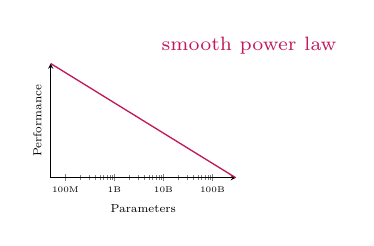
\begin{tikzpicture}[scale=0.60]
\begin{axis}[
    width=5.5cm, height=4cm,
    xlabel={\scriptsize Parameters},
    ylabel={\scriptsize Performance},
    xmode=log,
    axis lines=left,
    xtick={1e8, 1e9, 1e10, 1e11},
    xticklabels={\tiny 100M, \tiny 1B, \tiny 10B, \tiny 100B},
    ytick=\empty,
    xmin=5e7, xmax=3e11,
    no markers
]
\addplot[domain=5e7:3e11, samples=50, thick, neuronPink]
    {-0.3*ln(x/1e8) + 3.5};
\end{axis}
\node[font=\scriptsize, neuronPink] at (4.2,2.8) {smooth power law};
\end{tikzpicture}
\end{columns}

\vspace{0.2em}
\begin{insightbox}
\small Nobody fully understands why scale works this well. That is an open question.
\end{insightbox}

\note{
``GPT-1 had 117 million parameters. GPT-3 had 175 billion. Same transformer architecture. Same math. Just 1,500 times larger.

And somewhere along the way, these models started doing things nobody programmed: reasoning, writing code, translating languages they barely saw in training.

Kaplan showed in 2020 that performance scales as a smooth power law.

Nobody fully understands why scale works this well. That is an open question.''

Bridge: ``The machine that predicts `mat' from `The cat sat on the blank' is complete.''
}
\end{frame}

% ============================================================
% SLIDE 28: Inside the LLM -- ALL Building Blocks Found
% ============================================================
\begin{frame}{ALL Building Blocks Found}

\begin{columns}[T]
\column{0.55\textwidth}
\textbf{The transformer -- fully colored:}

\vspace{0.3em}
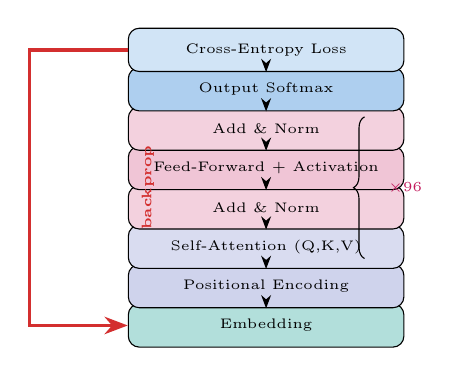
\begin{tikzpicture}[scale=0.50, every node/.style={font=\tiny}]
  \node[draw, fill=linalgTeal!30, rounded corners, minimum width=3.5cm, minimum height=0.55cm]
    (emb) at (0,0) {Embedding};
  \node[draw, fill=seqIndigo!25, rounded corners, minimum width=3.5cm, minimum height=0.55cm]
    (pos) at (0,1.0) {Positional Encoding};
  \node[draw, fill=seqIndigo!20, rounded corners, minimum width=3.5cm, minimum height=0.55cm]
    (attn) at (0,2.0) {Self-Attention (Q,K,V)};
  \node[draw, fill=neuronPink!20, rounded corners, minimum width=3.5cm, minimum height=0.55cm]
    (an1) at (0,3.0) {Add \& Norm};
  \node[draw, fill=neuronPink!25, rounded corners, minimum width=3.5cm, minimum height=0.55cm]
    (ff) at (0,4.0) {Feed-Forward + Activation};
  \node[draw, fill=neuronPink!20, rounded corners, minimum width=3.5cm, minimum height=0.55cm]
    (an2) at (0,5.0) {Add \& Norm};
  \node[draw, fill=probBlue!35, rounded corners, minimum width=3.5cm, minimum height=0.55cm]
    (out) at (0,6.0) {Output Softmax};
  \node[draw, fill=probBlue!20, rounded corners, minimum width=3.5cm, minimum height=0.55cm]
    (loss) at (0,7.0) {Cross-Entropy Loss};
  % Arrows
  \draw[-Stealth] (emb) -- (pos);
  \draw[-Stealth] (pos) -- (attn);
  \draw[-Stealth] (attn) -- (an1);
  \draw[-Stealth] (an1) -- (ff);
  \draw[-Stealth] (ff) -- (an2);
  \draw[-Stealth] (an2) -- (out);
  \draw[-Stealth] (out) -- (loss);
  % Backward
  \draw[-Stealth, very thick, calculusRed] (loss.west) -- +(-2.5,0) |- (emb.west);
  \node[calculusRed, font=\tiny\bfseries, rotate=90] at (-3.0,3.5) {backprop};
  % Brace
  \draw[decorate, decoration={brace, amplitude=4pt}] (2.5,1.7) -- (2.5,5.3)
    node[midway, right=5pt, font=\tiny\bfseries, neuronPink] {$\times 96$};
\end{tikzpicture}

\column{0.42\textwidth}
\vspace{0.5em}
\progressbar{5}

\vspace{0.5em}
\textbf{All five questions answered:}\\[6pt]
\textcolor{linalgTeal}{\faCheckSquare}~Similar words \textit{(vectors)}\\[2pt]
\textcolor{probBlue}{\faCheckSquare}~Choose next word \textit{(softmax)}\\[2pt]
\textcolor{calculusRed}{\faCheckSquare}~Learn from mistakes \textit{(backprop)}\\[2pt]
\textcolor{seqIndigo}{\faCheckSquare}~Understand context \textit{(attention)}\\[2pt]
\textcolor{neuronPink}{\faCheckSquare}~Get so good \textit{(depth + scale)}\\[8pt]

\small Every component has a name, a date, an inventor, and a topic where you learned why it matters.
\end{columns}

\note{
``Five questions. Five building blocks. Every component of the transformer has a name, a date, an inventor, and a topic where you learned why it matters.

The diagram that seemed overwhelming is now a map you can read.''

``Every time you type `The cat sat on the blank,' this entire machine activates. 2,000 years of mathematics, all running at once.''
}
\end{frame}

% ============================================================
% CLOSING  |  Slides 29--30
% ============================================================

% ============================================================
% SLIDE 29: Open Questions
% ============================================================
\begin{frame}{The Story Is Not Over}

\vspace{0.3em}

\begin{columns}[T]
\column{0.32\textwidth}
\begin{tcolorbox}[colframe=aiViolet, colback=aiViolet!5, boxrule=1pt,
  fonttitle=\bfseries\small, title={\faQuestion~Open Question 1}, left=3pt, right=3pt, top=3pt, bottom=3pt]
\small Why do transformers \textbf{generalize} so well?

\vspace{0.3em}
{\scriptsize They learn to write poetry from predicting the next word. Nobody fully understands why.}
\end{tcolorbox}

\column{0.32\textwidth}
\begin{tcolorbox}[colframe=aiViolet, colback=aiViolet!5, boxrule=1pt,
  fonttitle=\bfseries\small, title={\faQuestion~Open Question 2}, left=3pt, right=3pt, top=3pt, bottom=3pt]
\small What are the \textbf{limits} of scaling?

\vspace{0.3em}
{\scriptsize Does making it bigger always make it smarter? Where does it stop?}
\end{tcolorbox}

\column{0.32\textwidth}
\begin{tcolorbox}[colframe=aiViolet, colback=aiViolet!5, boxrule=1pt,
  fonttitle=\bfseries\small, title={\faQuestion~Open Question 3}, left=3pt, right=3pt, top=3pt, bottom=3pt]
\small What comes \textbf{after} transformers?

\vspace{0.3em}
{\scriptsize The transformer is 8 years old. Every major breakthrough we covered replaced what came before.}
\end{tcolorbox}
\end{columns}

\vspace{0.5em}

\begin{center}
\textit{Every breakthrough we covered started with someone asking a question nobody else was asking.}

\vspace{0.3em}
{\small The people who answer these questions \textbf{might be sitting in this room}.}
\end{center}

\note{
``The transformer is 8 years old. It was built from 2,000 years of math. Nobody fully understands why it works as well as it does.

There are open questions everywhere. And the people who answer them might be sitting in this room.''

The anchor has served its purpose. Now the student IS the anchor.
}
\end{frame}

% ============================================================
% SLIDE 30: Closing
% ============================================================
{
\setbeamercolor{background canvas}{bg=aiViolet}
\setbeamercolor{normal text}{fg=white}
\usebeamercolor[fg]{normal text}
\begin{frame}[plain]

\vspace{1.5cm}

\begin{center}
{\LARGE\textbf{\textcolor{white}{2,000+ Years. One Machine. Your Turn.}}}

\vspace{1.2em}

{\large\textcolor{white!90}{``The cat sat on the \rule{2cm}{0.5pt}''}}

\vspace{1.2em}

{\small\textcolor{white!80}{You now know every piece of the machine that answers this question.}}

\vspace{0.6em}

{\small\textcolor{white!80}{Grassmann was a schoolteacher. Pascal answered a gambling question.}}\\
{\small\textcolor{white!80}{Fourier studied heat. Boltzmann studied gas. Markov analyzed poetry.}}

\vspace{0.8em}

{\normalsize\textcolor{white!95}{They followed their curiosity and built the future.}}

\vspace{0.6em}

{\Large\textcolor{accentOrange}{\textbf{Your turn.}}}
\end{center}

\vspace{1cm}

\note{
``Every piece of mathematics we covered today was invented by someone who had no idea it would end up inside an AI.

Grassmann was a schoolteacher. Pascal was answering a gambling question. Fourier was studying heat. Boltzmann was studying gas molecules. Markov was analyzing poetry.

They followed their curiosity and built the future. Your turn.''

Final appearance of the anchor sentence. Closure.
}
\end{frame}
}

\end{document}
